% Options for packages loaded elsewhere
% Options for packages loaded elsewhere
\PassOptionsToPackage{unicode}{hyperref}
\PassOptionsToPackage{hyphens}{url}
\PassOptionsToPackage{dvipsnames,svgnames,x11names}{xcolor}
%
\documentclass[
  letterpaper,
  DIV=11,
  numbers=noendperiod]{scrartcl}
\usepackage{xcolor}
\usepackage{amsmath,amssymb}
\setcounter{secnumdepth}{-\maxdimen} % remove section numbering
\usepackage{iftex}
\ifPDFTeX
  \usepackage[T1]{fontenc}
  \usepackage[utf8]{inputenc}
  \usepackage{textcomp} % provide euro and other symbols
\else % if luatex or xetex
  \usepackage{unicode-math} % this also loads fontspec
  \defaultfontfeatures{Scale=MatchLowercase}
  \defaultfontfeatures[\rmfamily]{Ligatures=TeX,Scale=1}
\fi
\usepackage{lmodern}
\ifPDFTeX\else
  % xetex/luatex font selection
\fi
% Use upquote if available, for straight quotes in verbatim environments
\IfFileExists{upquote.sty}{\usepackage{upquote}}{}
\IfFileExists{microtype.sty}{% use microtype if available
  \usepackage[]{microtype}
  \UseMicrotypeSet[protrusion]{basicmath} % disable protrusion for tt fonts
}{}
\makeatletter
\@ifundefined{KOMAClassName}{% if non-KOMA class
  \IfFileExists{parskip.sty}{%
    \usepackage{parskip}
  }{% else
    \setlength{\parindent}{0pt}
    \setlength{\parskip}{6pt plus 2pt minus 1pt}}
}{% if KOMA class
  \KOMAoptions{parskip=half}}
\makeatother
% Make \paragraph and \subparagraph free-standing
\makeatletter
\ifx\paragraph\undefined\else
  \let\oldparagraph\paragraph
  \renewcommand{\paragraph}{
    \@ifstar
      \xxxParagraphStar
      \xxxParagraphNoStar
  }
  \newcommand{\xxxParagraphStar}[1]{\oldparagraph*{#1}\mbox{}}
  \newcommand{\xxxParagraphNoStar}[1]{\oldparagraph{#1}\mbox{}}
\fi
\ifx\subparagraph\undefined\else
  \let\oldsubparagraph\subparagraph
  \renewcommand{\subparagraph}{
    \@ifstar
      \xxxSubParagraphStar
      \xxxSubParagraphNoStar
  }
  \newcommand{\xxxSubParagraphStar}[1]{\oldsubparagraph*{#1}\mbox{}}
  \newcommand{\xxxSubParagraphNoStar}[1]{\oldsubparagraph{#1}\mbox{}}
\fi
\makeatother


\usepackage{longtable,booktabs,array}
\usepackage{calc} % for calculating minipage widths
% Correct order of tables after \paragraph or \subparagraph
\usepackage{etoolbox}
\makeatletter
\patchcmd\longtable{\par}{\if@noskipsec\mbox{}\fi\par}{}{}
\makeatother
% Allow footnotes in longtable head/foot
\IfFileExists{footnotehyper.sty}{\usepackage{footnotehyper}}{\usepackage{footnote}}
\makesavenoteenv{longtable}
\usepackage{graphicx}
\makeatletter
\newsavebox\pandoc@box
\newcommand*\pandocbounded[1]{% scales image to fit in text height/width
  \sbox\pandoc@box{#1}%
  \Gscale@div\@tempa{\textheight}{\dimexpr\ht\pandoc@box+\dp\pandoc@box\relax}%
  \Gscale@div\@tempb{\linewidth}{\wd\pandoc@box}%
  \ifdim\@tempb\p@<\@tempa\p@\let\@tempa\@tempb\fi% select the smaller of both
  \ifdim\@tempa\p@<\p@\scalebox{\@tempa}{\usebox\pandoc@box}%
  \else\usebox{\pandoc@box}%
  \fi%
}
% Set default figure placement to htbp
\def\fps@figure{htbp}
\makeatother





\setlength{\emergencystretch}{3em} % prevent overfull lines

\providecommand{\tightlist}{%
  \setlength{\itemsep}{0pt}\setlength{\parskip}{0pt}}



 


\usepackage{booktabs}
\usepackage{longtable}
\usepackage{array}
\usepackage{multirow}
\usepackage{wrapfig}
\usepackage{float}
\usepackage{colortbl}
\usepackage{pdflscape}
\usepackage{tabu}
\usepackage{threeparttable}
\usepackage{threeparttablex}
\usepackage[normalem]{ulem}
\usepackage{makecell}
\usepackage{xcolor}
\KOMAoption{captions}{tableheading}
\makeatletter
\@ifpackageloaded{caption}{}{\usepackage{caption}}
\AtBeginDocument{%
\ifdefined\contentsname
  \renewcommand*\contentsname{Table of contents}
\else
  \newcommand\contentsname{Table of contents}
\fi
\ifdefined\listfigurename
  \renewcommand*\listfigurename{List of Figures}
\else
  \newcommand\listfigurename{List of Figures}
\fi
\ifdefined\listtablename
  \renewcommand*\listtablename{List of Tables}
\else
  \newcommand\listtablename{List of Tables}
\fi
\ifdefined\figurename
  \renewcommand*\figurename{Figure}
\else
  \newcommand\figurename{Figure}
\fi
\ifdefined\tablename
  \renewcommand*\tablename{Table}
\else
  \newcommand\tablename{Table}
\fi
}
\@ifpackageloaded{float}{}{\usepackage{float}}
\floatstyle{ruled}
\@ifundefined{c@chapter}{\newfloat{codelisting}{h}{lop}}{\newfloat{codelisting}{h}{lop}[chapter]}
\floatname{codelisting}{Listing}
\newcommand*\listoflistings{\listof{codelisting}{List of Listings}}
\makeatother
\makeatletter
\makeatother
\makeatletter
\@ifpackageloaded{caption}{}{\usepackage{caption}}
\@ifpackageloaded{subcaption}{}{\usepackage{subcaption}}
\makeatother
\usepackage{bookmark}
\IfFileExists{xurl.sty}{\usepackage{xurl}}{} % add URL line breaks if available
\urlstyle{same}
\hypersetup{
  colorlinks=true,
  linkcolor={blue},
  filecolor={Maroon},
  citecolor={Blue},
  urlcolor={Blue},
  pdfcreator={LaTeX via pandoc}}


\author{}
\date{}
\begin{document}


\subsection{Weekly Assessment for Delta Operations on ESA and
CESA-listed
Osmerids}\label{weekly-assessment-for-delta-operations-on-esa-and-cesa-listed-osmerids}

Last updated: \emph{January 27, 2026}

\subsubsection{Executive Summary}\label{executive-summary}

\begin{itemize}
\tightlist
\item
  Entrainment management is currently active.
\item
  Delta smelt were detected at Chipps Island and the Sacramento Deep
  Water Ship Channel.
\item
  No Delta smelt or longfin smelt salvage has been observed this water
  year.
\item
  Turbidity in the central/south Delta is moderate.
\end{itemize}

\subsubsection{Operational and Regulatory
Conditions}\label{operational-and-regulatory-conditions}

\begin{itemize}
\tightlist
\item
  See current Weekly Fish and Water Operations Outlook document.
\item
  Additional information also available on the
  \href{https://www.cbr.washington.edu/sacramento/workgroups/delta_smelt.html}{SacPAS
  SMT page}.
\end{itemize}

\subsubsection{Delta smelt}\label{delta-smelt}

\paragraph{Biological}\label{biological}

\begin{itemize}
\item
  \textbf{Delta smelt life stages:} Adult
\item
  \textbf{Abundance estimate:} 258 (95\% CL: 16 to 1,219) as of the week
  of January 19--23, 2026
\item
  \textbf{Releases:} A total of 163,349 cultured Delta smelt have been
  released for WY 2026. The most recent release of 24,606 fish occurred
  in Sacramento River at Rio Vista on Dec 16, 2025.
\item
  \textbf{Delta smelt count:} 34 adult Delta smelt and 24 juvenile Delta
  smelt have been detected this water year. See
  Table~\ref{tbl-ds-recent-catch} for recent detections,
  Figure~\ref{fig-ds-map} for spatial distribution, and
  Figure~\ref{fig-ds-catch} for temporal distribution.
\item
  \textbf{Delta smelt salvage:} 0 Delta smelt have been salvaged, and
  the cumulative seasonal salvage is 0.
\end{itemize}

\textbf{Notes}

\begin{itemize}
\tightlist
\item
  Since there are few recent detections of Delta smelt, estimation of
  distribution within the Delta is limited.
\item
  As mentioned in EDSM reporting, fork length ranges reported for Delta
  smelt and longfin smelt life stages are defined by permit reporting
  purposes and are not intended to delineate cohorts or distinguish from
  hatchery or wild origin. See Table~\ref{tbl-ds-recent-catch} caption
  for fork-length ranges for age groups of Delta smelt.
\item
  See
  \href{https://www.cbr.washington.edu/sacramento/workgroups/delta_smelt.html}{SacPAS
  SMT Page} for additional details on releases and detection in surveys
  and salvage.
\item
  Historical salvage trends can be found at:
  \href{https://www.cbr.washington.edu/sacramento/data/query_salvage_hrt.html}{SacPAS
  Salvage Timing}
\end{itemize}

\begin{longtable}[]{@{}lllllr@{}}

\caption{\label{tbl-ds-recent-catch}Delta smelt detections in the last 2
weeks. Fork Length \textgreater{} 58mm = Adult, Fork Length 20-58mm =
Juvenile, Fork Length \textless{} 20mm = Larva.}

\tabularnewline

\toprule\noalign{}
Survey & Date & Region & Stratum & Life Stage & Catch \\
\midrule\noalign{}
\endhead
\bottomrule\noalign{}
\endlastfoot
EDSM & 2026-01-22 & North & Sac Deep Water & Adult & 1 \\

\end{longtable}

\begin{figure}[H]

\centering{

\pandocbounded{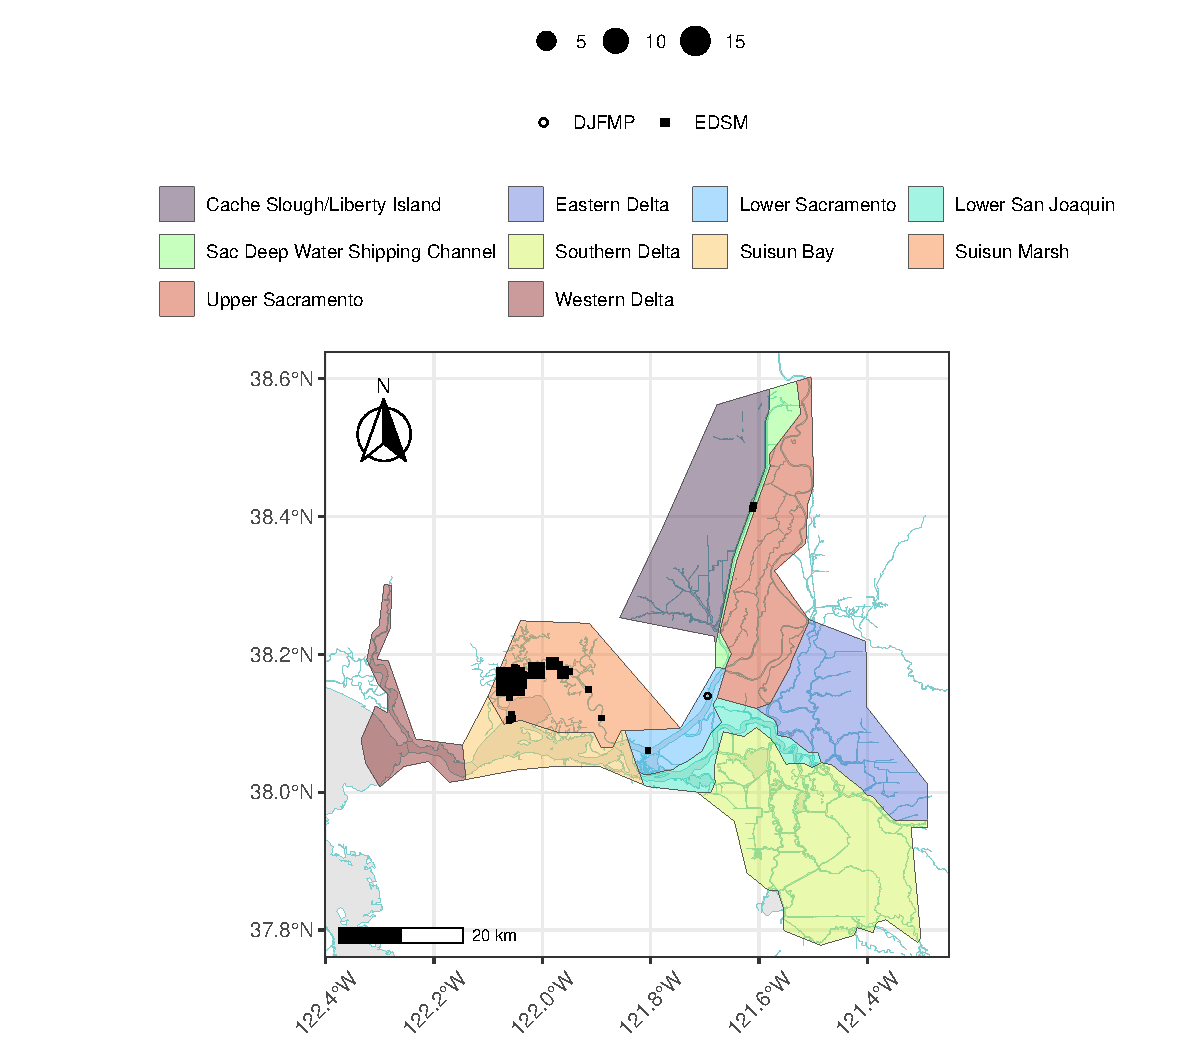
\includegraphics[keepaspectratio]{smt-assessment-v1_files/figure-pdf/fig-ds-map-1.pdf}}

}

\caption{\label{fig-ds-map}Delta smelt distribution for WY 2026}

\end{figure}%

\begin{longtable}[]{@{}lllr@{}}

\caption{\label{tbl-catch-all}Delta smelt water year totals by life
stage}

\tabularnewline

\toprule\noalign{}
Survey & Region & Life Stage & Total \\
\midrule\noalign{}
\endhead
\bottomrule\noalign{}
\endlastfoot
DJFMP & North & Juvenile & 1 \\
EDSM & North & Adult & 2 \\
EDSM & West & Adult & 32 \\
EDSM & West & Juvenile & 23 \\

\end{longtable}

\begin{figure}[H]

\centering{

\pandocbounded{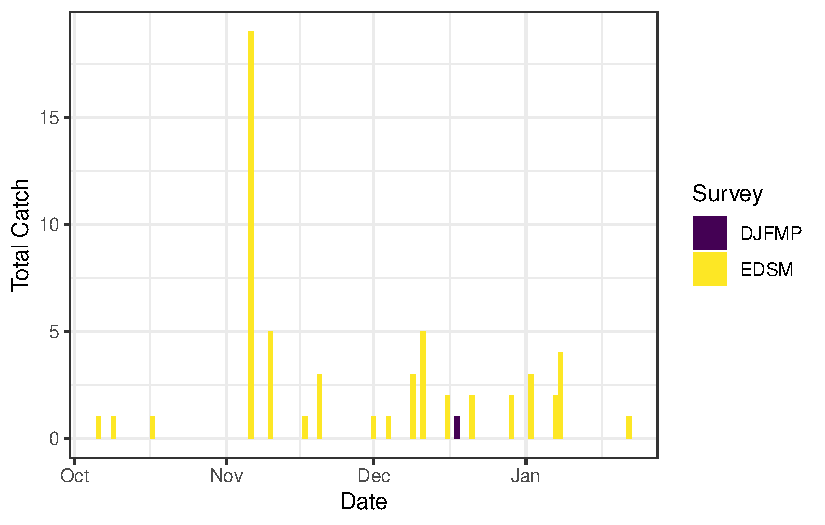
\includegraphics[keepaspectratio]{smt-assessment-v1_files/figure-pdf/fig-ds-catch-1.pdf}}

}

\caption{\label{fig-ds-catch}Time series of Delta smelt catch, WY 2026}

\end{figure}%

\paragraph{Environmental}\label{environmental}

\subparagraph{First Flush}\label{first-flush}

\begin{itemize}
\tightlist
\item
  Not relevant
\end{itemize}

\paragraph{Real-time Assessment
Thresholds}\label{real-time-assessment-thresholds}

\subparagraph{Adult Delta smelt}\label{adult-delta-smelt}

\textbf{Threshold}: If daily average JPF \textless{} 0 AND turbidity
\(\ge\) 12 FNU at OBI, HOL and OSJ

\begin{itemize}
\tightlist
\item
  \textbf{JPF}: 2,148 cfs as of Jan 25, 2026
\item
  \textbf{OBI Turbidity}: 6.49, 6.35, 5.97 FNU as of Jan 25, 2026
\item
  \textbf{HOL Turbidity}: 6.13, 6.19, 6.02 FNU as of Jan 25, 2026
\item
  \textbf{OSJ Turbidity}: 10.3, 9.74, 8.43 FNU as of Jan 25, 2026
\end{itemize}

\textbf{Offramp Adult Protections} when RVB or SJJ \textgreater{}
12\(^{\circ}\)C

\begin{itemize}
\tightlist
\item
  \textbf{RVB temperature (3-day average)}: 10.44\(^{\circ}\)C as of Jan
  25, 2026
\end{itemize}

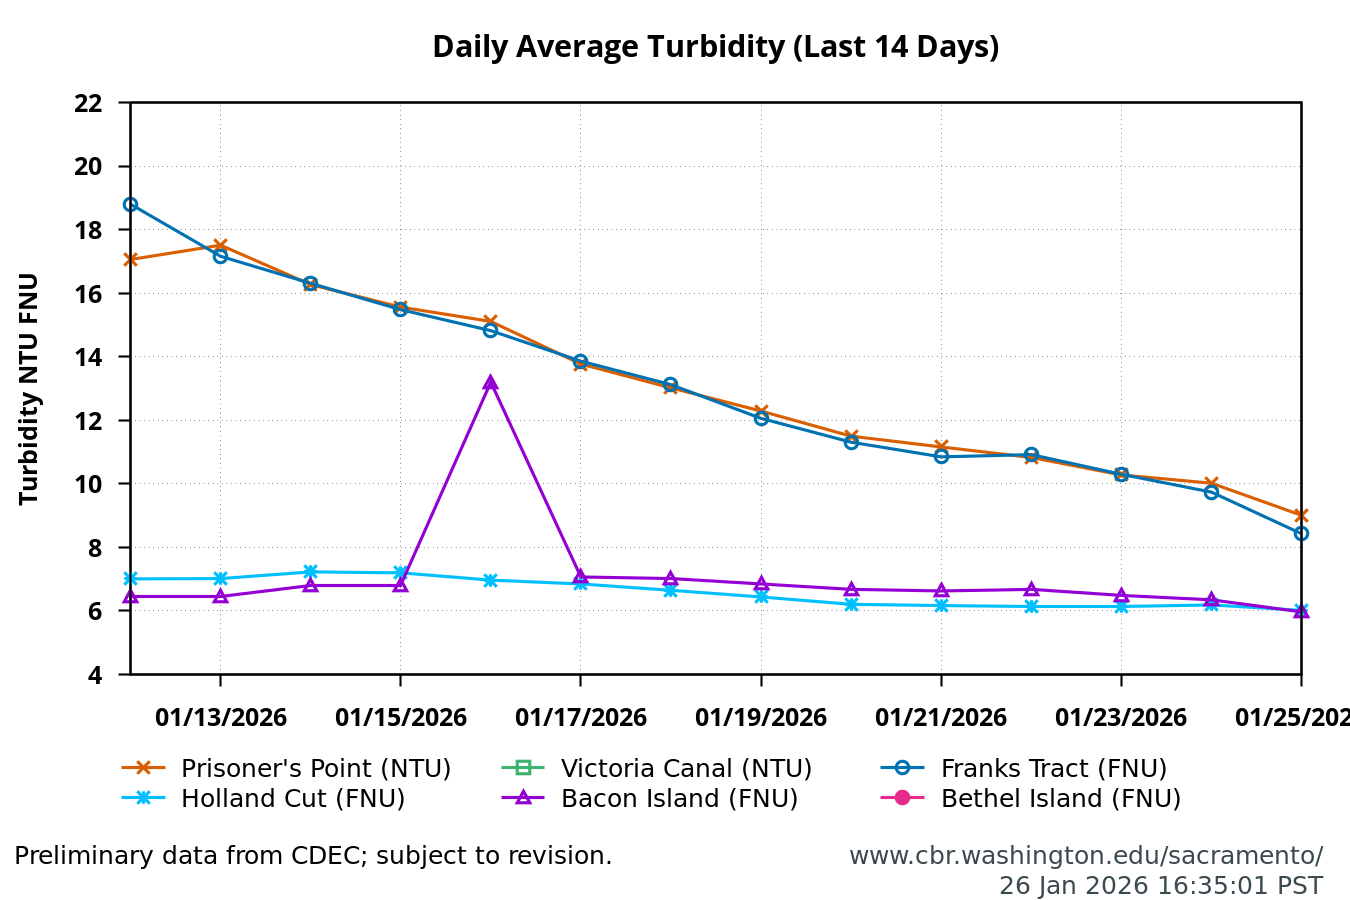
\includegraphics[width=0.85\linewidth,height=\textheight,keepaspectratio]{smelt_figures/freeport_turbidity.png}

\begin{itemize}
\tightlist
\item
  See
  \href{https://www.baydeltalive.com/current_conditions/constituent-tracker-turbidity}{Bay-Delta
  Live} for recent Delta-wide turbidity conditions.
\end{itemize}

\subparagraph{Larval/juvenile Delta
smelt}\label{larvaljuvenile-delta-smelt}

\textbf{Threshold}: After the onset of spawning, if JPF \textless{} 0
cfs AND turbidity is \(\ge\) 12 FNU in the south Delta AND PTM modeling
indicates the action would avoid \(\ge\) 5\% entrainment of Delta smelt
population after 30 days

\begin{itemize}
\tightlist
\item
  \textbf{12-station South Delta Turbidity}: The most recent average
  turbidity was 12.2 FNU as of Jan 13, 2025
\end{itemize}

\paragraph{Evaluation}\label{evaluation}

\textbf{Delta smelt:}

\begin{enumerate}
\def\labelenumi{\arabic{enumi}.}
\item
  After the start of entrainment management, is JPF \textless{} 0 and is
  daily average turbidity \(\ge\) 12 FNU in the OMR corridor (stations
  OBI, HOL, and OSJ)?

  No, these conditions will not be met this week.
\item
  Has the average water temperature at Jersey Point or Rio Vista not
  exceeded 53.6\(^{\circ}\)F (12\(^{\circ}\)C) for 3 consecutive days
  and/or has this action already been taken during WY 2026?

  Temperature at Rio Vista or Jersey Point has not exceeded the
  threshold. The Delta smelt adult entrainment management action has not
  yet been taken in WY 2026.
\item
  What is the evidence for the onset of Delta smelt spawning?

  Upstream migration for Delta smelt occurs between September and
  December and in response to ``first flush'' conditions (Sommer et
  al.~2011, Grimaldo et al.~2009). Migration typically ranges one to
  four weeks after flow and turbidity increases, based on salvage data
  (Sommer et al.~2011). Historically, detections of ripe Delta smelt
  began in January and peaked in February and March and the majority of
  Delta Smelt spawning occurs within a temperature range of 9-18˚C
  (Damon et al.~2016). Based on
  \href{https://github.com/Delta-Stewardship-Council/deltafish}{historical
  monitoring data} from the past few years, first detection of larvae in
  the Central and South Delta has typically occurred by mid to late
  March. Because first flush conditions were met on December 23, 2025,
  spawning may begin occurring during the current assessment week,
  consistent with the typical one- to four-week response window
  following increased flow and turbidity.Recent captures at Chipps
  Island and the Sacramento Deep Water Ship Channel are consistent with
  an upstream spawning migration into tidal freshwater habitats.
\item
  After the onset of spawning, have the following conditions occurred:
  \(\ge\) 5\% entrainment of the Delta smelt population at facilities
  after 30 days?

  Although spawning may occur during the current assessment period, JPF
  is above 0 cfs; therefore, the conditions required to evaluate larval
  and juvenile Delta smelt entrainment management are not met.
\end{enumerate}

\subsubsection{Longfin smelt}\label{longfin-smelt}

\paragraph{Biological}\label{biological-1}

\begin{itemize}
\item
  \textbf{Longfin smelt life stages:} Larva, Juvenile, Adult, NA
\item
  \textbf{Longfin smelt count:} 305 adult, 489 juvenile, and 446 larval
  longfin smelt have been detected this water year. See
  Table~\ref{tbl-lfs-recent-catch} for recent detections,
  Figure~\ref{fig-lfs-map} for spatial distribution, and
  Figure~\ref{fig-lfs-catch} for temporal distribution.
\item
  \textbf{Longfin smelt salvage:} 0 longfin smelt have been salvaged,
  and the cumulative seasonal salvage is 0.
\end{itemize}

\begin{longtable}[]{@{}lllllr@{}}

\caption{\label{tbl-lfs-recent-catch}Longfin smelt detections in the
last 2 weeks. Fork Length \textgreater{} 84mm = Adult, Fork Length
20-84mm = Juvenile, Fork Length \textless{} 20mm = Larva.}

\tabularnewline

\toprule\noalign{}
Survey & Date & Region & Stratum & Life Stage & Catch \\
\midrule\noalign{}
\endhead
\bottomrule\noalign{}
\endlastfoot
EDSM & 2026-01-20 & Far West & Suisun Bay & Adult & 4 \\
EDSM & 2026-01-20 & Far West & Suisun Bay & Juvenile & 29 \\
EDSM & 2026-01-20 & Far West & Suisun Bay & NA & 1 \\
EDSM & 2026-01-20 & West & Lower Sacramento & Adult & 1 \\
EDSM & 2026-01-22 & Far West & Western Delta & Juvenile & 1 \\
EDSM & 2026-01-26 & Far West & Suisun Bay & Adult & 4 \\
EDSM & 2026-01-26 & Far West & Suisun Bay & Juvenile & 11 \\
sls & 2026-01-14 & West & Lower San Joaquin & Larva & 2 \\
sls & 2026-01-14 & West & Suisun Bay & Larva & 5 \\

\end{longtable}

\begin{figure}[H]

\centering{

\pandocbounded{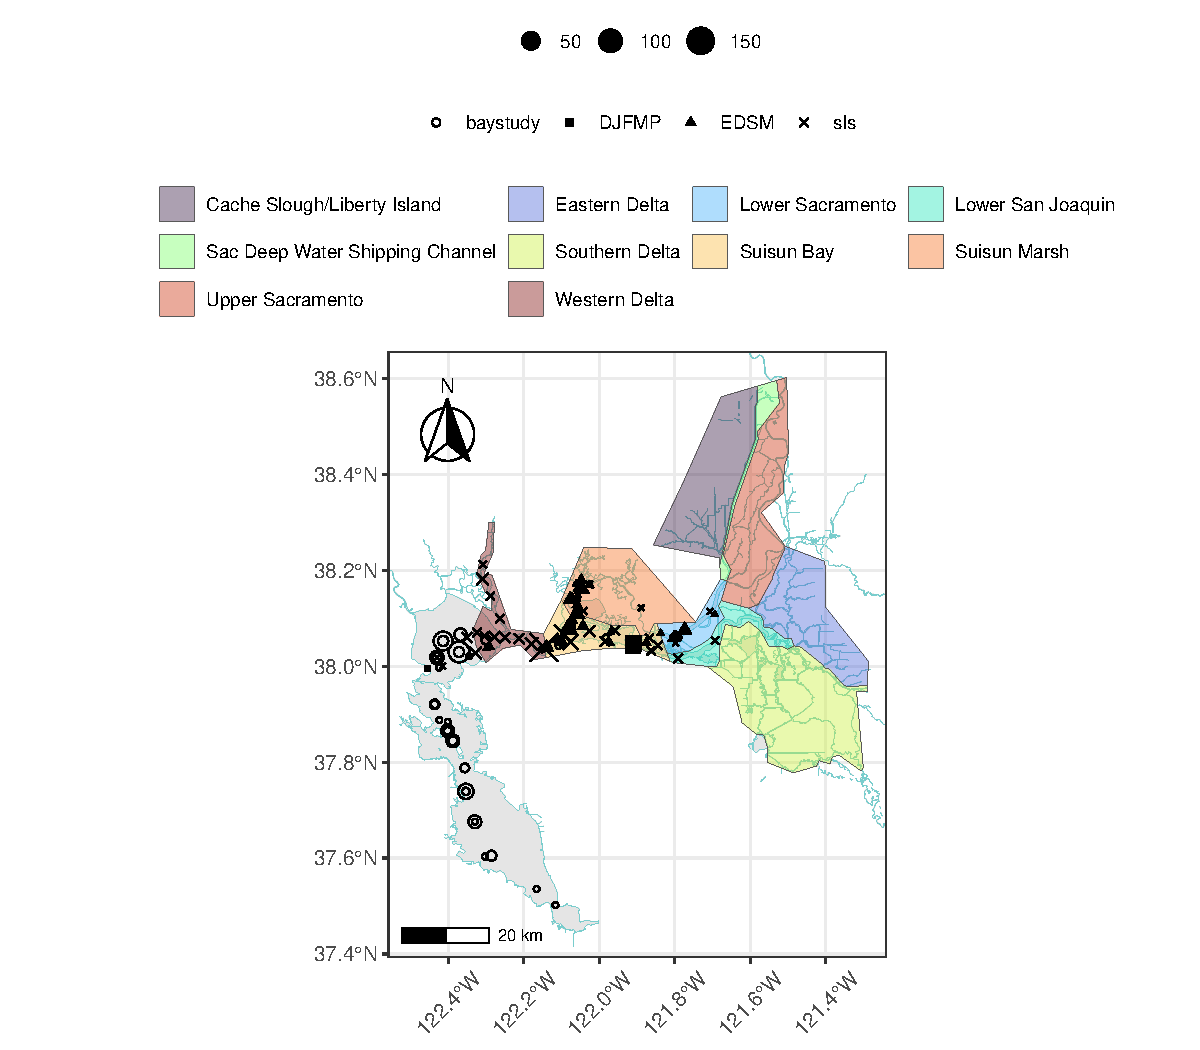
\includegraphics[keepaspectratio]{smt-assessment-v1_files/figure-pdf/fig-lfs-map-1.pdf}}

}

\caption{\label{fig-lfs-map}Longfin Smelt Distribution for WY 2026}

\end{figure}%

\begin{longtable}[]{@{}lllr@{}}

\caption{\label{tbl-lfs-catch-all}Longfin smelt water year totals by
life stage}

\tabularnewline

\toprule\noalign{}
Survey & Region & Life Stage & Total \\
\midrule\noalign{}
\endhead
\bottomrule\noalign{}
\endlastfoot
DJFMP & Bay & Juvenile & 1 \\
DJFMP & N/A & Adult & 240 \\
DJFMP & N/A & Juvenile & 14 \\
EDSM & Far West & Adult & 15 \\
EDSM & Far West & Juvenile & 56 \\
EDSM & North & Juvenile & 1 \\
EDSM & West & Adult & 42 \\
EDSM & West & Juvenile & 80 \\
baystudy & Bay & Adult & 6 \\
baystudy & Bay & Juvenile & 320 \\
baystudy & Far West & Adult & 2 \\
baystudy & Far West & Juvenile & 11 \\
baystudy & West & Juvenile & 6 \\
sls & Bay & Larva & 9 \\
sls & Far West & Larva & 349 \\
sls & North & Larva & 2 \\
sls & South & Larva & 2 \\
sls & West & Larva & 62 \\
sls & NA & Larva & 22 \\

\end{longtable}

\begin{figure}[H]

\centering{

\pandocbounded{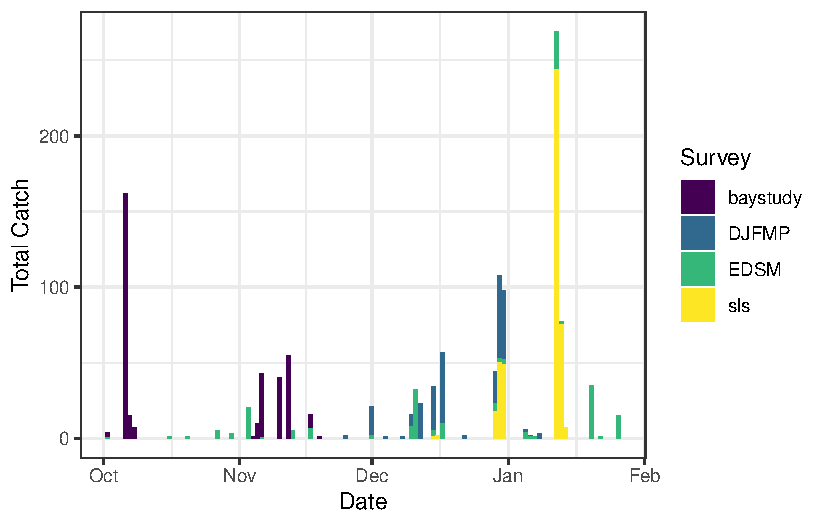
\includegraphics[keepaspectratio]{smt-assessment-v1_files/figure-pdf/fig-lfs-catch-1.pdf}}

}

\caption{\label{fig-lfs-catch}Time series of longfin smelt catch, WY
2026}

\end{figure}%

\paragraph{Real-time Assessment
Thresholds}\label{real-time-assessment-thresholds-1}

\subparagraph{Start of Entrainment Management (Adult Longfin
Smelt)}\label{start-of-entrainment-management-adult-longfin-smelt}

\begin{itemize}
\tightlist
\item
  Not relevant
\end{itemize}

\subparagraph{Adult longfin smelt}\label{adult-longfin-smelt}

\begin{itemize}
\tightlist
\item
  \textbf{Threshold:} JPF \textless{} 0 cfs, annual loss is on a
  trajectory to exceed 5\% of the adult population abundance, and
  reduced exports will reduce entrainment in the south Delta

  \begin{itemize}
  \tightlist
  \item
    Daily average JPF: 2,148 cfs as of Jan 25, 2026
  \item
    Adult abundance (Age 1+ LFS index): 2479.2 fish

    \begin{itemize}
    \tightlist
    \item
      5\% of abundance + 1: 125.0
    \end{itemize}
  \item
    Water year total adult longfin smelt salvage = 0
  \end{itemize}
\end{itemize}

\subparagraph{Larval/juvenile longfin
smelt}\label{larvaljuvenile-longfin-smelt}

\begin{itemize}
\tightlist
\item
  \textbf{Threshold:} JPF \textless{} 0 cfs AND population model
  demonstrates need to reduce entrainment to avoid population decline

  \begin{itemize}
  \tightlist
  \item
    Daily average JPF: 2,148 cfs as of Jan 25, 2026
  \end{itemize}
\end{itemize}

\paragraph{Evaluation}\label{evaluation-1}

\textbf{Longfin smelt:}

\begin{enumerate}
\def\labelenumi{\arabic{enumi}.}
\item
  If JPF \textless{} 0, what is the trajectory of annual loss of adult
  longfin smelt and is it likely to exceed 5\% of the adult population
  estimate? Is South Delta entrainment expected to decrease due to a
  reduction in export pumping?

  JPF is not \textless{} 0 cfs and no adult longfin smelt have been
  detected in salvage.
\item
  For larval and juvenile longfin smelt, if JPF \textless{} 0 cfs, do
  particle tracking models show a moderate to high difference in
  particle fates across different OMRI scenarios? Does Zone of Influence
  modeling show moderate to high changes in hydrodynamic footprint
  across different OMRI scenarios? Are these effects anticipated to
  cause a population decline?

  JPF is not \textless{} 0 cfs. ZOI modeling shows moderate change in
  the hydrodynamic footprint between OMRI scenarios, but no change
  between current and forecasted conditions.
\item
  Is there additional information or other analyses that should be
  considered in this evaluation?

  Additional information may be discussed if needed at the DAT call.
\end{enumerate}

\subsubsection{End of smelt Entrainment
Management}\label{end-of-smelt-entrainment-management}

\begin{itemize}
\tightlist
\item
  Not relevant
\end{itemize}

\subsubsection{References}\label{references}

Damon, L. J., S. B. Slater, R. D. Baxter, and R. W. Fujimura. 2016.
Fecundity and reproductive potential of wild female Delta smelt in the
upper San Francisco Estuary, California. California Fish and Game
102(4):188--210.

Grimaldo, L. F., T. Sommer, N. Van Ark, G. Jones, E. Holland, P. B.
Moyle, B. Herbold \& P. Smith (2009) Factors Affecting Fish Entrainment
into Massive Water Diversions in a Tidal Freshwater Estuary: Can Fish
Losses be Managed? North American Journal of Fisheries Management, 29:5,
1253-1270, DOI: 10.1577/M08-062.1

Sommer, T., F. Mejia, M. Nobriga, and L. Grimaldo. 2011. The Spawning
Migration of Delta Smelt in the Upper San Francisco Estuary. San
Francisco Estuary and Watershed Science 9(2).




\end{document}
